% chktex-file 44 32 36 38 18 11 8 26

\pagestyle{DS_FP}
%\NomPrenomNote{}

\bigskip


\subsection*{Contexte général}

Une entreprise spécialisée dans les systèmes embarqués développe un nouveau module de transmission de données sans fil. Les équipes travaillent sur trois problématiques distinctes: la modélisation du signal de charge d'un condensateur, la gestion d'une mémoire tampon (buffer), et le contrôle qualité des modules produits.

\section*{PARTIE A~--~Contrôle de qualité}

\medskip

\emph{Dans cette partie, vous arrondirez toutes les valeurs à $10^{-4}$ si nécessaire.}

\medskip

 \begin{minipage}{0.48\textwidth}
L'usine produit des modules de transmission. Le service qualité distingue deux lignes de production:

\begin{itemize}
    \item la ligne A, qui produit $60\%$ des modules et génère $3\%$ de défectueux;
    \item la ligne B, qui produit $40\%$ des modules et génère $7\%$ de défectueux.
\end{itemize}

On note $D$ l'événement « le module est défectueux », $A$ l'événement « le module provient de la ligne A » et $B$ l'événement « le module provient de la ligne B ».

Un module est prélevé au hasard en sortie de chaîne.

\medskip

\begin{enumerate}[series=monDS, resume]
    \item Compléter l'arbre de probabilité ci-contre.
\end{enumerate}

\end{minipage}\hfill{}
\begin{minipage}{0.48\textwidth}
    \begin{blocvisiblex}[height=6]
    {\begin{center}
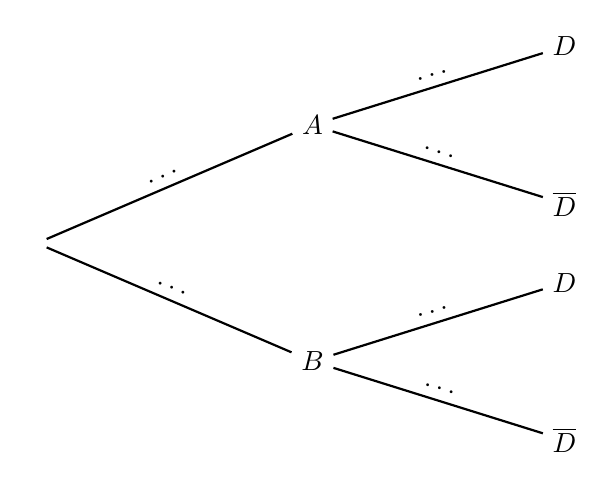
\begin{tikzpicture}[
    grow=right,     % On définit la croissance vers la droite
    % Réglages des distances entre les niveaux et les branches
    level 1/.style={sibling distance=3cm, level distance=3.5cm},
    level 2/.style={sibling distance=2cm, level distance=3.2cm},
    every node/.style={sloped}, % Aligne le texte sur les branches
    edge from parent/.style={draw, thick} % Ajoute une flèche au bout
]
% Racine
\node {} 
    child { node {$B$}
        child { node {$\overline{D}$} 
            edge from parent node[above] {$\ldots{}$} }
        child { node {$D$} 
            edge from parent node[above] {$\ldots{}$} }
        edge from parent node[above] {$\ldots{}$} }
    child { node {$A$}
        child { node {$\overline{D}$} 
            edge from parent node[above] {$\ldots{}$} }
        child { node {$D$} 
            edge from parent node[above] {$\ldots{}$} }
        edge from parent node[above] {$\ldots{}$} }
    ;
\end{tikzpicture}
\end{center}}
\begin{center}
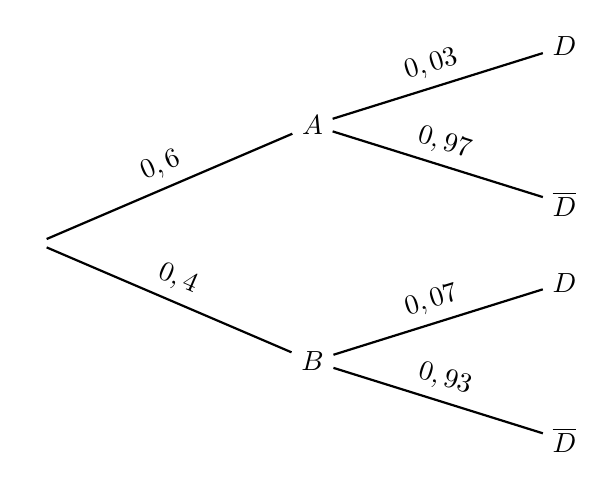
\begin{tikzpicture}[
    grow=right,     % On définit la croissance vers la droite
    % Réglages des distances entre les niveaux et les branches
    level 1/.style={sibling distance=3cm, level distance=3.5cm},
    level 2/.style={sibling distance=2cm, level distance=3.2cm},
    every node/.style={sloped}, % Aligne le texte sur les branches
    edge from parent/.style={draw, thick} % Ajoute une flèche au bout
    %edge from parent/.style={draw, -latex, thick} % Ajoute une flèche au bout
]
% Racine
\node {} 
    child { node {$B$}
        child { node {$\overline{D}$} 
            edge from parent node[above] {$0,93$} }
        child { node {$D$} 
            edge from parent node[above] {$0,07$} }
        edge from parent node[above] {$0,4$} }
    child { node {$A$}
        child { node {$\overline{D}$} 
            edge from parent node[above] {$0,97$} }
        child { node {$D$} 
            edge from parent node[above] {$0,03$} }
        edge from parent node[above] {$0,6$} }
    ;
\end{tikzpicture}
\end{center}
    \end{blocvisiblex}
\end{minipage}



    
\begin{enumerate}[resume=monDS]
    \item Calculer la probabilité que le module prélevé soit défectueux et provienne de la ligne A.
     \begin{blocvisiblex}[height=2.5]
    {\quad}
    $P(A\cap D)=P(A) \times P_D(A)=0,6 \times 0,03=0,018$

    \smallskip
    La probabilité que le module prélevé soit défectueux et provienne de la ligne A est de $0,018$.
     \end{blocvisiblex}
     \medskip
    \item Montrer que la probabilité que le module prélevé soit défectueux est égale à \fbox{$0,046$}.
    \begin{blocvisiblex}[height=2.5]
    {\quad}
    $P(D)=P(A\cap D)+P(B\cap D)=P(A) \times P_D(A)+P(B) \times P_D(B)=0,6 \times 0,03+0,4 \times 0,07=0,046$

        \smallskip
    La probabilité que le module prélevé soit défectueux est de $0,046$.
    \end{blocvisiblex}
    \medskip
    \item Calculer $P_D(A)$ et donner une interprétation de cette valeur dans le contexte de l'exercice.
    \begin{blocvisiblex}[height=2.5]
    {\quad}
    $P_D(A)=\dfrac{P(A\cap D)}{P(D)}=\dfrac{P(A) \times P_D(A)}{P(D)}=\dfrac{0,6 \times 0,03}{0,046}\approx 0,3913$

        \smallskip
    La probabilité que le module provienne de la ligne A sachant qu'il est défectueux est d'environ $0,3913$.
     \end{blocvisiblex}
     \medskip
     
\end{enumerate}

Un technicien prélève un échantillon de \fbox{30} modules indépendamment les uns des autres. On admet que la probabilité qu'un module soit défectueux est \fbox{$0,046$}

Soit $X$ la variable aléatoire qui compte le nombre de modules défectueux dans l'échantillon. On supposera que cette variable aléatoire suit une loi binomiale.

\begin{enumerate}[series=monDS, resume]

\begin{minipage}{0.47\textwidth}
        \item Donner les paramètres de cette loi binomiale
\end{minipage}\hfill{}
\begin{minipage}{0.47\textwidth}
    \begin{blocvisiblex}[height=1]
    {\quad}
    $n=30$ et $p=0,046$
    \end{blocvisiblex}
\end{minipage}


\begin{minipage}{0.47\textwidth}
    \bigskip
    \item Déterminer la probabilité qu'au moins 2 modules soient défectueux dans l'échantillon.
\end{minipage}\hfill{}
\begin{minipage}{0.47\textwidth}
    \begin{blocvisiblex}[height=1]
    {\quad}
    $P(X\geq 2)= 0.4043$
    \end{blocvisiblex}
\end{minipage}
\end{enumerate}

\pagebreak
Le technicien souhaite que la probabilité de détecter au moins un module défectueux sur $n$ prélèvements soit supérieure à \fbox{$0,9$}.

\begin{enumerate}[series=monDS, resume]
    \item Montrer que cette condition s'écrit \fbox{${0,954}^n \leq 0,1$}.
    \begin{blocvisiblex}[height=3]
    {\quad}
    $P(X\geq 1)=1-P(X=0)=1-{(1-p)}^n=1-{0,954}^n$

    La condition $P(X\geq 1)\geq0,99$ s'écrit alors $1-{(1-p)}^n\geq 0,9$ soit ${0,954}^n \leq 0,1$.
    \end{blocvisiblex}
    \medskip
    \begin{minipage}{0.50\textwidth}
    \item A l'aide de Géogébra, déterminer à partir de quel valeur de $n$ la condition est satisfaite.
\end{minipage}\hfill{}
\begin{minipage}{0.43\textwidth}
    \begin{blocvisiblex}[height=1]
    {$n=\dotfill$}
    $n= 49$
    \end{blocvisiblex}
\end{minipage}

    \appelprof{}
\end{enumerate}

\medskip

\section*{PARTIE B~--~Modélisation du signal de charge d'un condensateur}

Un ingénieur modélise la tension aux bornes d'un condensateur lors d'une phase de charge par une fonction de la forme:

\[\boxed{f(t)=(at+b)\cdot \e^{-kt}}\qquad \text{où $a$, $b$ et $k$ sont des constantes réelles.}\]

\begin{itemize}
    \item $t$ est le temps en millisecondes (ms) depuis le début de la charge du condensateur.
    \item $f(t)$ est la tension en volts (V) aux bornes du condensateur à l'instant $t$.
    \item $k$ est un coefficient de décroissance qui modélise la résistance du circuit, influençant la rapidité avec laquelle la tension atteint son maximum et commence à décroître.
\end{itemize}

\subsection*{Etude d'un cas particulier}

    Dans cette partie uniquement, on considèrera que les constantes $a$, $b$ et $k$ prennent les valeurs suivantes:

    \begin{minipage}{0.28\textwidth}
\begin{itemize}
    \item $a=0$,
    \item $b=5$,
    \item $k=0,5$.
\end{itemize}
\end{minipage}\hfill{}
\begin{minipage}{0.68\textwidth}
    Ainsi la fonction $f$ s'exprime par: \fbox{$f(t)=5\cdot \e^{-0,5t}$}.

\end{minipage}



\begin{enumerate}[series=monDS, resume]
    \item Déterminer par le calcul une expression de la fonction dérivée $f'$ et montrer que \fbox{$f'(t)=-\dfrac{5}{2}\cdot \e^{-0,5t}$}.
    \begin{blocvisiblex}[height=2.8]
    {\quad}
    $f(t)= 5 \cdot \e^{-0,5t}$

    $f'(t)= 5 \cdot \Big(-0,5\cdot \e^{-0,5t}\Big)=-\dfrac{5}{2}\cdot \e^{-0,5t}$.
    \end{blocvisiblex}
    \medskip
    \item En déduire les variations de $f$ sur $\fo{0}{+\infty}$.
    \begin{blocvisiblex}[height=3]
    {\quad}
    $f'(t)$ est strictement négatif sur $\fo{0}{+\infty}$, ainsi $f$ est strictement décroissante sur $\fo{0}{+\infty}$.
    \end{blocvisiblex}

\end{enumerate}


\subsection*{Modélisation}

Dans cette partie, on considère que $a$, $b$ et $k$ sont des constantes réelles strictement positives, mais on ne connaît pas leurs valeurs.

Des études expérimentales ont permis de déterminer que:
\begin{itemize}
    \item la tension initiale $f(0)$ est de $5$ volts;
    \item la tension atteint un maximum au bout de $1,5$ ms.
    \item le coefficient de décroissance $k$ est égal à $0,5$.
\end{itemize}

La fonction $f$ est donc définie pour tout $t\geqslant 0$ par \fbox{$f(t)=(at+b)\cdot \e^{-0,5t}$}

\bigskip

\begin{enumerate}[series=monDS, resume]
    \begin{minipage}{0.48\textwidth}
    \item A l'aide des deux conditions expérimentales et à l'aide de Géogébra, déterminer les valeurs de $a$ et $b$.
\end{minipage}\hfill{}
\begin{minipage}{0.45\textwidth}
    \begin{blocvisiblex}[height=1.2]
    {$a=\dotfill \hspace{2cm} b=\dotfill$}
    $a=10 \hspace{2cm} b=5$
    \end{blocvisiblex}
\end{minipage}
    \appelprof{}
\end{enumerate}

\bigskip

Dans la suite de l'exercice on considèrera la fonction $f$ définie sur $\fo{0}{+\infty}$ par \fbox{$f(t)=5\cdot (2t+1)\cdot \e^{-0,5t}$}.

\begin{enumerate}[series=monDS, resume]
    \begin{minipage}{0.46\textwidth}
            \item Déterminer grâce à Géogébra l'expression factorisée de la fonction dérivée $f'$.

    \end{minipage}\hfill{}
    \begin{minipage}{0.48\textwidth}
\begin{blocvisiblex}[height=1.5]
    {\quad}

    \[f'(t)= \dfrac{5}{2}\cdot \Big(2t-3\Big)\cdot \e^{-0,5t}\]


    \end{blocvisiblex}
    \end{minipage}
    
    \medskip
    
    \item Déterminer par le calcul le signe de la fonction dérivée $f'(t)$ et compléter le tableau de variations de $f$ sur $\fo{0}{+\infty}$.
    \begin{blocvisiblex}[height=5.5]
    {
    \begin{minipage}{0.48\linewidth}
        \quad
    \end{minipage}\hfill{}
    \begin{minipage}{0.46\linewidth}
        \begin{tikzpicture}
                \tkzTabInit[lgt=1.8,espcl=2.3]
                {$t$ / 1, signe $\, f'(t)$ / 1, var \, $f$ / 2}
                {$0$,$\quad$, $+\infty$}
                \tkzTabLine{}
                \tkzTabVar{}
            \end{tikzpicture}
    \end{minipage}
    }
        \begin{minipage}{0.48\linewidth}
        $\e^{-0,5t}$ est strictement positif sur l'ensemble de définition. Ainsi le signe de $f'(t)$ est celui de $-\dfrac{5}{2}\big(2t-3\big)$.

        $2t-3$ est négatif sur $\fo{0}{1,5}$, nul en $t=1,5$ et positif sur $\fo{1,5}{+\infty}$.
    
        $f$ est donc croissante sur $\fo{0}{1,5}$, décroissante sur $\fo{1,5}{+\infty}$ et atteint un minimum en $t=1,5$.
    \end{minipage}\hfill{}
    \begin{minipage}{0.46\linewidth}
\begin{tikzpicture}
                \tkzTabInit[lgt=1.8,espcl=2.3]
                {$t$ / 1, signe $\, f'(t)$ / 1, var \, $f$ / 2}
                {$0$, ${1,5}$, $+\infty$}
                \tkzTabLine{,+,z,-,}
                \tkzTabVar{-/ $5$, +/ ${f(1,5)}$, -/ $0$}
            \end{tikzpicture}
        \end{minipage}
\end{blocvisiblex}
\end{enumerate}

\medskip


\begin{enumerate}[series=monDS, resume]
     
   \item Déterminer grâce à Géogébra à partir de quelle valeur de $t$ la tension $f(t)$ devient inférieure à 1 volt. (On donnera une valeur approchée à $10^{-2}$ près.)
    \begin{blocvisiblex}[height=1]
    {\quad}
    $f(t)<1$ à partir de $t\approx 9,14$ ms.
    \end{blocvisiblex}
\end{enumerate}

L'énergie dissipée en \textbf{joules} entre l'instant $a$ et l'instant $b$ est égal à $E=\displaystyle \int_{a}^{b} f(t) \dt$.

\begin{enumerate}[series=monDS, resume]
    \begin{minipage}{0.46\textwidth}
            \item Déterminer une primitive $F$ de $f$ sur $\fo{0}{+\infty}$.
    \end{minipage}\hfill{}
    \begin{minipage}{0.46\textwidth}
        \begin{blocvisiblex}[height=1.2]
    {\quad}

    \[F(t)=-10\cdot (2t+5)\cdot \e^{-0,5t}\]
    \end{blocvisiblex}
    \end{minipage}
    
    \medskip

    \item La fonction $F$ étant une primitive de $f$, quelle expression permet de calculer l'énergie $E$ dissipée entre l'instant $a$ et l'instant $b$? Cocher la bonne réponse:
   \begin{blocvisiblex}[height=1]
    {
    \faSquare[regular] \, $F(a) - F(b)$ \hfill \faSquare[regular] \, $F(b) - F(a)$ \hfill \faSquare[regular] \, $F(b)$ \hfill \faSquare[regular] \, $F(a)$ \hspace{1cm} 
 }         
    \faSquare[regular] \, $F(a) - F(b)$ \hfill \faCheck[regular] \, $F(b) - F(a)$ \hfill \faSquare[regular] \, $F(b)$ \hfill \faSquare[regular] \, $F(a)$ \hspace{1cm} 
    \end{blocvisiblex}
    \medskip
\item On suppose maintenant que l'énergie dissipée pendant les 5 premières milliseconde est égale à 40 joutes. Déterminer par le calcul l'énergie moyenne $\mu$ dissipée par milliseconde pendant les 5 premières millisecondes.
    \begin{blocvisiblex}[height=3]
    {\quad}
    L'énergie moyenne dissipée par milliseconde pendant les 5 premières millisecondes est $\mu=\dfrac{1}{5} \times 40=8$ joutes par milliseconde.
    \end{blocvisiblex}
    \medskip
    
\end{enumerate}
    

\bigskip

\thispagestyle{DS_LP}

%\thispagestyle{DS_LP}
\section*{PARTIE C~--~Gestion d'une mémoire tampon}

Un buffer (mémoire tampon) contient initialment 200 octets de données. A chaque cycle d'horloge, le système traite et supprime $10\%$ du contenu actuel du buffer.

On note $u_n$ la quantité de données (en octets) présente dans le buffer après $n$ cycles d'horloge.

\begin{enumerate}[series=monDS, resume]
    \item Justifier que la suite $(u_n)$ vérifie la relation de récurrence $u_{n+1}=0,9\cdot u_n$.
    \begin{blocvisiblex}[height=3.5]
    {\quad}
    La suite $(u_n)$ vérifie la relation de récurrence $u_{n+1}=0,9\cdot u_n$ car à chaque cycle d'horloge, le système traite et supprime $10\%$ du contenu actuel du buffer

    On a donc $u_{n+1}=u_n-0,1\cdot u_n=0,9\cdot u_n$.

    \end{blocvisiblex}
    \medskip
    \item Déterminer la nature de la suite $(u_n)$. 
    \begin{blocvisiblex}[height=2]
    {\quad}

    La suite $(u_n)$ est de la forme $u_{n+1}=q \times u_n$ avec $q=0,9$ constant, donc c'est une suite géométrique de raison $0,9$ et de premier terme $u_0=200$.
    \end{blocvisiblex}
    \medskip
    \item Exprimer $u_n$ en fonction de $n$. 
    \begin{blocvisiblex}[height=2]
    {\quad}
    $(u_n)$ est une suite géométrique de raison $0,9$ et de premier terme $u_0=200$, donc pour tout $n$ entier naturel, on a $u_n=u_0 \times q^n=200 \times 0,9^n$.
    \end{blocvisiblex}
    \medskip
    \begin{minipage}{0.45\textwidth}
    \item Compléter l'algorithme ci-dessous qui calcule le nombre de cycles d'horloges nécessaires pour que la quantité de données dans le buffer soit inférieure à 1 octet.

    \end{minipage}\hfill{}
    \begin{minipage}{0.46\textwidth}
    \begin{tcblisting}{%
  listing only,
  colback=white, 
  colupper=black, 
  title=Algorithme de recherche de seuil,
  boxsep=0pt,
  left=5mm,
  listing options={
    numbers=none,
    basicstyle=\ttfamily,
    escapeinside={(*}{*)},
    literate={<-}{{$\bm{\leftarrow}$}}2, % Ajout d'un petit espace après la flèche
    frame=none % Supprime le cadre interne de listings
    }
}
n <- 0
u <- 200
tant que (*\trou{u >= 1}*):
        u <- (*\trou{0,9 * u}*)
        n <- (*\trou{n + 1}*)
print(n)
\end{tcblisting}
    \end{minipage}
    \medskip

    \begin{minipage}{0.70\textwidth}
            \item Par la méthode de votre choix, déterminer le nombre de cycles d'horloge nécessaires pour que la quantité de données dans le buffer soit inférieure à 1 octet.
    \end{minipage}\hfill{}
    \begin{minipage}{0.20\textwidth}
\begin{blocvisiblex}[height=1.2]
{\quad}
  $n=51$
    \end{blocvisiblex}
    \end{minipage}
    
\end{enumerate}

\bigskip



